\documentclass[a4paper]{article}
\usepackage{graphicx}
\usepackage{amsmath, amsfonts, geometry, float, listings, enumerate, multicol}
\usepackage{multicol, float, color, colortbl}
\usepackage{tikz, titlesec, parskip, pgfplots, filecontents}
\usepackage{hyperref}
\usepackage{amsmath}
\usepackage{tikz, titlesec, parskip}
\usepackage{tikz,pgfplots}
\usepackage[americanvoltages,fulldiodes,siunitx]{circuitikz}
\usetikzlibrary{shapes,arrows}
\usepackage{enumitem}
\titleformat*{\subsubsection}{\LARGE\bfseries}

\titlespacing{\section}{0pt}{10pt}{0pt}
\titlespacing{\subsection}{0pt}{10pt}{0pt}
\titlespacing{\subsubsection}{0pt}{10pt}{0pt}



\usetikzlibrary{calc,patterns,through}
\newcommand{\arcangle}{%
	\mathord{<\mspace{-9mu}\mathrel{)}\mspace{2mu}}%
}

\renewcommand{\baselinestretch}{1.4}
 \geometry{
 a4paper,
 total={170mm,257mm},
 left=20mm,
 top=20mm,
 }
\usepackage{fancyhdr}
\usepackage{indentfirst}
\pagestyle{fancy}
\fancyhf{}
\rhead{\textbf{بهینه‌سازی در علوم داده}}
\lhead{\textbf{ تمرین پنجم}}
\cfoot{(\space \space \space \space \textbf{\thepage}  \space \space \space)}
\renewcommand{\headrulewidth}{1pt}
\renewcommand{\footrulewidth}{1pt}

 
\usepackage{xepersian}
\setlatintextfont{Times New Roman}
\settextfont{XB Niloofar}
\setdigitfont{XB Niloofar}
\DefaultMathsDigits

\makeatletter
\bidi@patchcmd{\@Abjad}{آ}{الف}
{\typeout{Succeeded in changing آ into الف}}
{\typeout{Failed in changing آ into الف}}
\makeatother
\PersianAlphs

\begin{document}
\begin{minipage}{0.6\textwidth}
\begin{bf}
\begin{center}
	\large
	به نام خدا\\
دکتر مجتبی تفاق - بهینه‌سازی در علوم داده \\
\Large
\vspace{0.4cm}
امیرحسین جوادی (97101489)
\end{center}
\end{bf}
\normalsize
\end{minipage} \hfill
\begin{minipage}{0.35\textwidth}
\begin{flushleft}
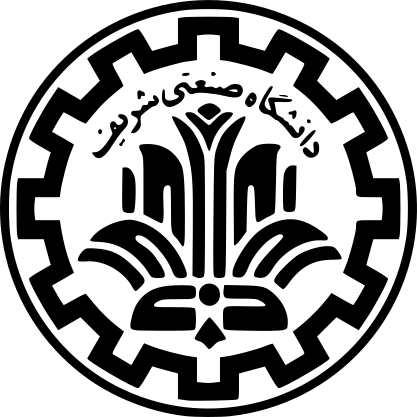
\includegraphics[width=0.5\textwidth]{logo.png}
\end{flushleft}
\begin{flushleft}
	دانشگاه صنعتی شریف\\
	دانشکده مهندسی برق\\
\end{flushleft}

\end{minipage}
\\
\rule[0.1\baselineskip]{\textwidth}{1pt}
\begin{latin}
\section{2.8 Polyhedra}
Which of the following sets $ S $ are polyhedra? If possible, express $ S $ in the form $ S = \{x | Ax \preceq b, F x = g\} $.
\begin{enumerate}
	\item $ S = \{y_{1}a_{1} + y_{2}a_{2} | −1 \leq y_{1} \leq 1, −1 \leq y_{2} \leq 1\} $, where $ a_{1}, a_{2} \in R^{n} $.
	\item $ S = \{x \in R^{n} | x \succeq 0, 1^{T} x = 1, \sum_{i=1}^{n} x_{i} a_{i} = b_{1}, \sum_{i=1}^{n} x_{i} a_{i}^{2} = b_{2}\} $, where
	$ a_{1}, \dots , a_{n} \in R$ and $b_{1}, b_{2} \in R $.
	\item $ S = \{x \in R^{n} | x \succeq 0, x^{T} y \leq 1$ for all $ y $ with $ ||y||_{2} = 1\} $.
	\item $ S = \{x \in R^{n} | x \succeq 0, x^{T} y \leq 1$ for all $ y $ with $ \sum_{i=1}^{n} |y_{i}| = 1\}$.
\end{enumerate}
\textcolor{red}{\textbf{Solution:}}
\begin{enumerate}
	\item It is polyhedra. It is the Affine mapping of $ \hat{S} = \{y | −1 \leq y_{1} \leq 1, −1 \leq y_{2} \leq 1\} $. For more illustration: 
	\begin{equation*}
		z = \begin{bmatrix} 
			z_{1} \\
			z_{2} \\
			\vdots \\
			z_{n}
		\end{bmatrix} = 
		\begin{bmatrix} 
			a_{1}^{1} & a_{1}^{2} \\
			a_{2}^{1} & a_{2}^{2} \\
			\vdots & \vdots\\
			a_{n}^{1} & a_{n}^{2} 
		\end{bmatrix}
		\begin{bmatrix} 
			y_{1} \\
			y_{2} \\
		\end{bmatrix}
	\end{equation*}
	Now, we should figure out how conditions on $ y $ act on $ z $.
	\item It is polyhedra. For $ S $ form, $ A = -I_{n \times n} $, $ b = 0_{n \times 1} $, and 
	\begin{equation*}
		F = \begin{bmatrix} 
			1 & 1 & 1 & \dots & 1 \\
			a_{1} & a_{2} & a_{3} & \dots & a_{n} \\
			a_{1}^{2} & a_{2}^{2} & a_{3}^{2} & \dots & a_{n}^{2}
		\end{bmatrix}
		\qquad
		g = \begin{bmatrix} 
			1 \\
			b_{1}\\
			b_{2}
		\end{bmatrix}
	\end{equation*}
	\item It is not a polyhedra. $ x \succeq 0, x^{T} y \leq 1$ for all $ y $ with $ ||y||_{2} = 1  \Leftrightarrow ||x||_{2} \leq 1 $. So the final result is the intersection of the unit ball and the nonnegative orthant $ R_{n}^{+} $. We can not see $ S $ as the intersection of finite halfspaces and hyperplane.
	\item  It is a polyhedra. First we should prove that $ x^{T} y \leq 1$ for all $ y $ with $ \sum_{i=1}^{n} |y_{i}| = 1 \Leftrightarrow |x_{i}| \leq 1 $ for $ i = 1, 2, \dots n$.
	\\
	Right to left:
	\begin{equation*}
		x^T y = \sum_{i} x_{i} y_{i} \leq \sum_{i} |x_{i}| |y_{i}| \leq \sum_{i}  |y_{i}| = 1
	\end{equation*}
	Left to right:
	\begin{equation*}
		x_{k} = \max(|x_{i}|) \Rightarrow
		y = e_{k} \times sign(x_{k}) \Rightarrow x^T y = \sum_{i} x_{i} y_{i} = x_{k} y_{k} = |x_{k}| \Rightarrow |x_{i}| \leq 1 \text{ for } i = 1, 2, \dots n.
	\end{equation*}
	This can be defined by the intersection of nonnegative orthant $ R_{n}^{+} $ with $ \{x | -1 \preceq x \preceq 1\} $.  For $ S $ form
	\begin{equation*}
		A = \begin{bmatrix} 
			1 & 0 & \dots & 0\\
			0 & 1 & \dots & 0\\
			\vdots & \vdots & \vdots & \vdots \\
			0 & 0 & \dots & 1\\
			-1 & 0 & \dots & 0\\
			0 & -1 & \dots & 0\\
			\vdots & \vdots & \vdots & \vdots \\
			0 & 0 & \dots & -1\\
			1 & 0 & \dots & 0\\
			0 & 1 & \dots & 0\\
			\vdots & \vdots & \vdots & \vdots \\
			0 & 0 & \dots & 1\\
		\end{bmatrix}
		\; \; 
		b = \begin{bmatrix} 
			1 \\
			1 \\
			\vdots \\
			1 \\
			1\\
			1 \\
			\vdots \\
			1 \\
			0 \\
			0 \\
			\vdots \\
			0 \\
		\end{bmatrix}
	\end{equation*}
\end{enumerate}
\section{2.9 Voronoi sets and polyhedral decomposition}
Let $ x_{0}, x_{1}, \dots , x_{K} \in R^{n} $ Consider the set of
points that are closer (in Euclidean norm) to $ x_{0} $ than the other $ x_{i} $, i.e.,
\begin{equation*}
	V = \{x \in R^{n} | \; ||x - x_{0}||_{2} \leq ||x - x_{i}||_{2}, i = 1, \dots , K\}.
\end{equation*}
$ V $ is called the Voronoi region around $ x_{0} $ with respect to $ x_{1}, \dots , x_{K} $.
\begin{enumerate}
	\item Show that $ V $ is a polyhedron. Express $ V $ in the form $ V = \{x | Ax \preceq b\} $.
	\item Conversely, given a polyhedron $ P $ with nonempty interior, show how to find $ x_{0}, \dots , x_{K} $ so that the polyhedron is the Voronoi region of $ x_{0} $ with respect to $ x_{1}, \dots , x_{K} $.
	\item We can also consider the sets
	\begin{equation*}
		V_{k} = \{x \in R^{n}| \; ||x - x_{k}||_{2} \leq ||x - x_{i}||_{2}, i \neq k\}.
	\end{equation*}
	The set $ V_{k} $ consists of points in $ R^{n} $ for which the closest point in the set $ \{x_{0}, \dots , x_{K}\} $ is $ x_{k} $.
	\\
	The sets $ V_{0}, . . . , V_{K} $ give a polyhedral decomposition of $ R^{n} $. More precisely, the sets $ V_{k} $ are polyhedra, $ \bigcup_{k=1}^{K} V_{k} = R^{n} $, and  $ \text{int } V_{i} \cap \text{int } V_{j} = \emptyset $ for $ i \neq j $, i.e., $ V_{i} $ and $ V_{j} $ intersect at most along a boundary.
	\\
	Suppose that $ P_{1}, \dots , P_{m} $ are polyhedra such that $ \bigcup_{i=1}^{m} P_{i} = R^{n} $,  and  $ \text{int } P_{i} \cap \text{int } P_{j} = \emptyset $ for $ i \neq j $. Can this polyhedral decomposition of $ R_{n} $ be described as the Voronoi regions generated by an appropriate set of points?
\end{enumerate}
\textcolor{red}{\textbf{Solution:}}
\begin{enumerate}
	\item For every $ i \neq j $, we have a hyperspace where every point on the hyperplane has less or equal distance to $ x_{i} $ than $ x_{j} $. This hyperspace includes the point $ \frac{x_{i} + x_{j}}{2} $ and its normal vector is $ x_{j} - x_{i} $. So for every point of $ \{x_{1}, x_{2}, \dots, x_{k}\} $,  we have a hyperspace $ \{h_{1}, h_{2}, \dots, h_{k}\} $ that in every hyperspace like $ h_{i} $, the distance of any points to $ x_{0} $ is less than its distance to $ x_{i} $. Each hyperspace can be written in the form below:
	\begin{equation*}
		\begin{cases}
		h_{i}: \{x \in R^{n} | a_{i}^{T} x \leq b_{i}\} \\
		a_{i} = x_{i} - x_{0} \\
		b_{i} = a_{i}^{T}(\dfrac{x_{0} + x_{i}}{2})\\
		\end{cases}
	\end{equation*}
	The intersection of these hyperspace is our final result. So we can write it as below:
	\begin{gather*}
		V = \{ x \in R^{n} | Ax\preceq b\}
		\\
		A = \begin{bmatrix}
			a_{1}^{T}\\
			a_{2}^{T}\\
			\vdots \\
			a_{n}^{T}
		\end{bmatrix}
		\qquad
		b = \begin{bmatrix}
			b_{1}\\
			b_{2}\\
			\vdots \\
			b_{n}	
		\end{bmatrix}	
	\end{gather*}
	\item
	Suppose we have $ V = \{x | Ax \preceq b\} $. This polyhedron is the intersection of $ K $ hyperspaces. Each hyperspace has the form $ a_{i}^{T} x \leq b_{i} $ which $ a_{i}^{T} $ is the $ i $'th row of $ A $ and $ b_{i} $ is the i'th element of $ b $. $ x_{0} $ can be any point in $ V $ and each $ x_{i} $ is the mirror image of $ x_{0} $ with respect to the hyperplane $ a_{i}^{T} x = b_{i} $.
	\item 
	No, this can be a counter example.
	\begin{center}
			\begin{tikzpicture}
			\draw (-4,0) -- (4,0) node[above]{$L_1$};
			\draw (-3.4,-2) -- (3.4,2) node[above]{$L_2$};
			\filldraw (2,0.6) circle (2pt) node[anchor=west]{$ P_{1} $};
			\filldraw (-2,-0.6) circle (2pt) node[anchor=east]{$ P_{2} $};
			\filldraw[gray] (1.4,1.4) circle (2pt) node[anchor=west]{$ P_{3} $};
			\filldraw[gray] (-2,0.6) circle (2pt) node[anchor=east]{$ P_{3}' $};
		\end{tikzpicture}
	\end{center}
	By selecting $ P_{1} $ in hyperspace between of $L_1$ and $L_2$ and $ R_{++} $, $ P_{2} $ should be the mirror point of $ P_{1} $ with respect to the origin. The third point can not be computed because the mirror image of $ P_{1} $ with respect to $L_2$ ($ P_{3} $) is not the same of the mirror image of $ P_{2} $ with respect to $L_1$ ($ P_{3}' $).
\end{enumerate}
\section{2.15 Some sets of probability distributions}
Some sets of probability distributions. Let $ x $ be a real-valued random variable with $ \mathbb{P}(x = a_{i}) = p_{i}, i = 1, \dots , n $, where $ a_{1} < a_{2} < \dots < a_{n} $. Of course $ p \in R^{n} $ lies in the standard probability simplex $ P = \{p | 1^{T} p = 1, p \succeq 0\} $. Which of the following conditions are convex in $ p $? (That is, for which of the following conditions is the set of $ p \in P $ that satisfy the condition convex?)
\begin{enumerate}
	\item $ \alpha \leq \mathbb{E}f(x) \leq \beta $, where $ \mathbb{E}f(x) $ is the expected value of $ f(x) $, i.e., $ \mathbb{E}f(x) = \sum_{i=1}^{n}  p_{i}f(a_{i}) $. (The  function $ f : R \rightarrow R $ is given.)
	\item $ \mathbb{P}(x > \alpha) \leq \beta $.
	\item $ \mathbb{E} |x^{3}| \leq \alpha E |x| $.
	\item  $ \mathbb{E} x^{2} \leq \alpha $.
	\item  $ \mathbb{E} x^{2} \geq \alpha $.
	\item  var($ x $) $ \geq \alpha $, where var($ x $) = $\mathbb{E}( x - \mathbb{E}x )^{2}$ is the variance of $ x $.
	\item  var($ x $) $ \leq \alpha $.
	\item  quartile($ x $) $ \geq \alpha $, where quartile($ x $) = $ \inf\{\beta | \mathbb{P}(x \leq \beta) \geq 0.25\} $.
	\item  quartile($ x $) $ \leq \alpha $.
\end{enumerate}
\textcolor{red}{\textbf{Solution:}}
\begin{enumerate}
	\item $ \mathbb{E}f(x) = \sum_{i=1}^{n}  p_{i}f(a_{i}) $ is a weighted sum of $  p_{i} $, so $ \mathbb{E}f(x) \geq \alpha $ and $ \mathbb{E}f(x) \leq \beta $ are two hyperspaces. So the final result is the intersection of two halfspaces and a polyhedron. As a result, it is still convex. 
	\item Imagine $ \alpha < a_{k} $ and  $ \alpha \geq a_{k-1} $. So $ \mathbb{P}(x > \alpha) \leq \beta $ is equal to $ \sum_{i=k}^{n} p_{i} \leq \beta $. 
	\begin{equation*}
		\begin{bmatrix}
			0_{1 \times (k-1)} & 1_{1 \times (n-k+1)}
		\end{bmatrix}  P \leq \beta
	\end{equation*}
	The answer is the intersection of P and the halfspace described above. So it is still convex.
	\item $ \mathbb{E} |x^{3}| \leq \alpha E |x| $ is equal to $ \mathbb{E} (|x^{3}|-\alpha|x|) \leq 0 $. $ \mathbb{E} (|x^{3}|-\alpha|x|) \leq 0 $ is a weighted sum of $  p_{i} $, so  $ \mathbb{E} (|x^{3}|-\alpha|x|) \leq 0 $ is a hyperspace. So the final result is the intersection of a halfspace and a polyhedron. As a result, it is still convex.  
	\item  $ \mathbb{E}x^{2} = \sum_{i=1}^{n} p_{i} a_{i}^{2} $ is a weighted sum of $  p_{i} $, so $ \mathbb{E}x^{2} \leq \alpha $ is a hyperspace. So the final result is the intersection of a halfspace and a polyhedron. As a result, it is still convex. 
	\item  $ \mathbb{E}x^{2} = \sum_{i=1}^{n} p_{i} a_{i}^{2} $ is a weighted sum of $  p_{i} $, so $ \mathbb{E}x^{2} \geq \alpha $ is a hyperspace. So the final result is the intersection of a halfspace and a polyhedron. As a result, it is still convex. 
	\item  Counter example: with $ n=2, a_{1}=0, a_{2}=1 $ 
	\begin{center}
		Case1 : $ p_{1}=1, p_{2}=0 \Rightarrow var(x) = \frac{1}{4} $ \\
		Case2 : $ p_{1}=0, p_{2}=1 \Rightarrow var(x) = \frac{1}{4} $ \\
		Case3 : $ p_{1}=0.5, p_{2}=0.5 \Rightarrow var(x) = 0 $
	\end{center}
	So by taking $ \alpha < \frac{1}{4} $, the convex combination of Case1 and Case2 is not in the set. So it is not convex.
	\item  It is convex
	\begin{gather*}
		var(x) = \sum_{i=1}^{n} p_{i} a_{i}^{2} - (\sum_{i=1}^{n} p_{i} a_{i})^{2} \Rightarrow var(x) \leq \alpha \Rightarrow \sum_{i=1}^{n} p_{i} a_{i}^{2} - (\sum_{i=1}^{n} p_{i} a_{i})^{2} \leq \alpha
		\\
		b = [a_{1}^{2}, a_{2}^{2}, \dots, a_{n}^{2}]_{n \times 1}, A = a a^{T} \Rightarrow b^{T}p - p^{T} A p \leq \alpha
		\\
		\forall p_{1},p_{2} \in \{P | var(P) \leq \alpha \} \Rightarrow b^{T}p_{1} - p_{1}^{T} A p_{1} \leq \alpha \text{ and } b^{T}p_{2} - p_{2}^{T} A p_{2} \leq \alpha
		\\
		p3 = \theta_{1}p_{1} + \theta_{2}p_{2} \text{ with } \theta_{1},\theta_{2} \geq 0, \theta_{1}+\theta_{2} = 1
		\\
		var(p_{3}) = b^{T}p_{3} - p_{3}^{T} A p_{3} = b^{T}(\theta_{1}p_{1} + \theta_{2}p_{2}) - (\theta_{1}p_{1} + \theta_{2}p_{2})^{T} A (\theta_{1}p_{1} + \theta_{2}p_{2}) 
		\\
		= \theta_{1} b^{T}p_{1} + \theta_{2} b^{T}p_{2} - \theta_{1}^{2} p_{1}^{T}Ap_{1} - \theta_{1} \theta_{2} p_{1}^{T}Ap_{2} - \theta_{1} \theta_{2} p_{2}^{T}Ap_{1} - \theta_{2}^{2} p_{2}^{T}Ap_{2}
		\\
		\leq \theta_{1} (\alpha + p_{1}^{T}Ap_{1}) + \theta_{2} (\alpha + p_{2}^{T}Ap_{2}) - \theta_{1}^{2} p_{1}^{T}Ap_{1} - \theta_{1} \theta_{2} p_{1}^{T}Ap_{2} - \theta_{1} \theta_{2} p_{2}^{T}Ap_{1} - \theta_{2}^{2} p_{2}^{T}Ap_{2} 
		\\
		= \alpha + \theta_{1} p_{1}^{T}Ap_{1} + \theta_{2} p_{2}^{T}Ap_{2} - \theta_{1}^{2} p_{1}^{T}Ap_{1} - \theta_{1} \theta_{2} p_{1}^{T}Ap_{2} - \theta_{1} \theta_{2} p_{2}^{T}Ap_{1} - \theta_{2}^{2} p_{2}^{T}Ap_{2} \leq \alpha
		\end{gather*}
	The last in equality comes from the fact that:
	\begin{gather*}
		z = \max(p_{1}^{T}Ap_{1}, p_{2}^{T}Ap_{2}, p_{1}^{T}Ap_{2})
		\\
		\theta_{1} p_{1}^{T}Ap_{1} + \theta_{2} p_{2}^{T}Ap_{2} - \theta_{1}^{2} p_{1}^{T}Ap_{1} - \theta_{1} \theta_{2} p_{1}^{T}Ap_{2} - \theta_{1} \theta_{2} p_{2}^{T}Ap_{1} - \theta_{2}^{2} p_{2}^{T}Ap_{2} \leq \theta_{1} z + \theta_{2} z - \theta_{1}^{2} z - \theta_{1} \theta_{2} z - \theta_{1} \theta_{2} z - \theta_{2}^{2} z \leq 0
	\end{gather*}
	This is obvious by putting $ \theta_{1} = 1 - \theta_{2} $.
	\item This means that $ \mathbb{P}(x \leq \beta) < 0.25 \text{ for all } \beta < \alpha $. if $ \alpha < a_{1} $, $ \mathbb{P}(x \leq \beta) = 0 $ and it is always true. Otherwise we have a set like $ \{ a_{1}, a_{2}, \dots, a_{k} \}$ that its member are all less that $ \alpha $. So for the condition $ \mathbb{P}(x \leq \beta) < 0.25 \text{ for all } \beta < \alpha $ we should have:
	\begin{equation*}
		\sum_{i=1}^{k} \mathbb{P}(p_{i}) < 0.25
	\end{equation*}
	which is a linear inequality. So it is convex.
	\item Same as previous, this time we need
	\begin{equation*}
		\sum_{i=k+1}^{n} \mathbb{P}(p_{i}) > 0.25
	\end{equation*}
	which is a linear inequality. So it is convex.
\end{enumerate}
\section{2.17 Image of polyhedral sets under perspective function}
In this problem we study the image of hyperplanes, halfspaces, and polyhedra under the perspective function $ P(x, t) = x/t $, with dom $ P = R^{n} \times R_{++} $. For each of the following sets $ C $, give a simple description of
\begin{equation*}
	P(C) = \{v/t | (v, t) \in C, t > 0\}
\end{equation*}
\begin{enumerate}
	\item The polyhedron $ C = \text{conv}\{(v_{1}, t_{1}), \dots , (v_{K}, t_{K})\} $ where $ v_{i} \in R^{n}  $ and $ t_{i} > 0 $.
	\item 
	The hyperplane $ C = \{(v, t) | f^{T} v + gt = h\} $ (with $ f $ and $ g $ not both zero).
	\item
	The halfspace $ C = \{(v, t) | f^{T} v + gt \leq h\} $ (with $ f $ and $ g $ not both zero).
	\item 
	The polyhedron $ C = \{(v, t) | Fv + gt \preceq h\} $.	
\end{enumerate}
\textcolor{red}{\textbf{Solution:}}
\begin{enumerate}
	\item
	Every $ (x,y) \in C $ can be written in form below:
	\begin{gather*}
		x = a_{1} v_{1} + a_{2} v_{2} + \dots +  a_{K} v_{K} 
		\\
		y = a_{1} t_{1} + a_{2} t_{2} + \dots +  a_{K} t_{K} 
		\\
		P(x,y) = \frac{x}{y} = \frac{\sum_{i=1}^{K} a_{i} v_{i}}{\sum_{i=1}^{K} a_{i} t_{i}} = \sum_{i=1}^{K} \frac{a_{i} t_{i}}{\sum_{i=1}^{K} a_{i} t_{i}} \frac{v_{i}}{t_{i}}
		\\
		\sum_{i=1}^{K} \frac{a_{i} t_{i}}{\sum_{i=1}^{K} a_{i} t_{i}} = 1 \Rightarrow \text{ Convex combination of } \{\frac{v_{i}}{t_{i}}\}
		\\
		P(x,y) \subseteq \text{conv}\{\frac{v_{1}}{t_{1}}, \frac{v_{2}}{t_{2}}, \dots , \frac{v_{K}}{t_{K}} \}
	\end{gather*}
	We need to show that $ \text{conv}\{\frac{v_{1}}{t_{1}}, \frac{v_{2}}{t_{2}}, \dots , \frac{v_{K}}{t_{K}} \}  \subseteq P(x,y) $ too.
	\begin{gather*}
		\frac{x'}{y'} = b_{1} \frac{v_{1}}{t_{1}} + b_{2} \frac{v_{2}}{t_{2}} + \dots + b_{K} \frac{v_{K}}{t_{K}}
	\end{gather*}
	We can see that $ P(x,y) = \frac{x'}{y'} $ with $ x $ and $ y $ to be:
	\begin{gather*}
		b_{i} = \frac{a_{i} t_{i}}{\sum_{i=1}^{K} a_{i} t_{i}} \Rightarrow a_{i} = \frac{b_{i}}{t_{i}} \sum_{i=1}^{K} a_{i} t_{i} = \frac{b_{i}}{t_{i} \sum_{i=1}^{K} \frac{b_{i}}{ t_{i}} }
	\end{gather*}
	We can see that $ x $ and $ y $ can be written in form below.
	\begin{gather*}
		x = a_{1} v_{1} + a_{2} v_{2} + \dots +  a_{K} v_{K} 
		\\
		y = a_{1} t_{1} + a_{2} t_{2} + \dots +  a_{K} t_{K} 
	\end{gather*}
	So  $ \text{conv}\{\frac{v_{1}}{t_{1}}, \frac{v_{2}}{t_{2}}, \dots , \frac{v_{K}}{t_{K}} \}  \subseteq P(x,y) $. 
	As a result  $ P(C) = \text{conv}\{\frac{v_{1}}{t_{1}}, \frac{v_{2}}{t_{2}}, \dots , \frac{v_{K}}{t_{K}} \} $
	\item 
	\begin{gather*}
		f^{T} v + gt = h \Rightarrow f^{T} \frac{v}{t} + g = \frac{h}{t} \Rightarrow f^{T} x + g = \frac{h}{t} 
		\\
		P(C) = \begin{cases}
			\{x | f^{T} x + g > 0\} & h>0 \\
			\{x | f^{T} x + g = 0\} & h=0 \\
			\{x | f^{T} x + g < 0\} & h<0 \\
		\end{cases}
	\end{gather*}
	\item 
	\begin{gather*}
		f^{T} v + gt \leq h \Rightarrow f^{T} \frac{v}{t} + g \leq \frac{h}{t} \Rightarrow f^{T} x + g \leq \frac{h}{t} 
		\\
		P(C) = \begin{cases}
			R^{n} & h>0 \\
			\{x | f^{T} x + g \leq 0\} & h=0 \\
			\{x | f^{T} x + g < 0\} & h<0 \\
		\end{cases}
	\end{gather*}
	\item 
	\begin{gather*}
		Fv + gt \preceq h \Rightarrow F \frac{v}{t} + g \preceq \frac{h}{t} \Rightarrow Fx + g \preceq \frac{h}{t} 
	\end{gather*}
	For this, $ (Fx + g)_{i} $ and $ h_{i} $ should be both negative or both positive. Then we can find a $ t $ to reach our inequality.
	\begin{gather*}
		P(C) = \{ x | Fx + g \preceq \frac{h}{t} \text{ for a } t>0 \}
		\\
		\begin{cases}
			(Fx + g)_{i} \leq 0 & h_{i}=0 \\
			(Fx + g)_{i}< 0 & h_{i}<0 \\
		\end{cases}
	\end{gather*}
	Another important point is to find a $ t $. For negative $ h_{i} $ we tend to have big $ t $ and for positive  $ h_{i} $ we tend to have small $ t $. So we need to have another constrain. 
	\begin{gather*}
		\dfrac{(Fx + g)_{i}}{h_{i}} \leq \dfrac{(Fx + g)_{j}}{h_{j}} \text{ for every $ i $ with } h_{i}>0 \text{ and every $ j $ with } h_{j}<0
	\end{gather*}
\end{enumerate}
\section{2.31 Properties of dual cones}
Let $ K^{*} $ be the dual cone of a convex cone $ K $, as defined in (2.19). Prove the following.
\begin{enumerate}
	\item $ K^{*} $ is indeed a convex cone.
	\item $ K_{1} \subseteq K_{2} $ implies $ K_{2}^{*} \subseteq K_{1}^{*} $.
	\item $ K^{*} $ is closed.
	\item The interior of $ K^{*} $ is given by int $ K^{*} = \{y | y^{T} x > 0 \text{ for all } x \in \text{cl } K \}$.
	\item If $ K $ has nonempty interior then $ K^{*} $ is pointed.
	\item $ K^{**} $ is the closure of $ K $. (Hence if $ K $ is closed,  $ K^{**} = K $.)
	\item If the closure of $ K $ is pointed then $ K^{*} $ has nonempty interior.
\end{enumerate}
\textcolor{red}{\textbf{Solution:}}
\begin{enumerate}
	\item for every $ y_{1},y_{2} \in K^{*}$, we need to prove $ w = \theta_{1} y_{1} + \theta_{2} y_{2} $ for every $ \theta_{1},\theta_{2}>0 $ is in $ K^{*} $.
	\begin{equation*}
		w^{T}x = (\theta_{1} y_{1} + \theta_{2} y_{2})^{T}x = \theta_{1} y_{1}^{T}x + \theta_{2} y_{2}^{T}x > 0 \Rightarrow w \in K^{*}
	\end{equation*}
	\item 
	We should prove that every $ y \in K_{2}^{*} $ is in $ K_{1}^{*} $.
	\begin{equation*}
		y \in K_{2}^{*}	\Rightarrow y^{T}x \geq 0 \text{ for all } x \in K_{2} \Rightarrow y^{T}x \geq 0 \text{ for all } x \in K_{1} \Rightarrow y \in K_{1}^{*}
	\end{equation*}
	\item 
	$ K^{*} $ is the intersection of a set of homogeneous halfspaces including the origin. Hence it is a closed convex cone.
	\item 
	$ y $ is in the interior of a convex space $ K^{*} $ if every point in $ B(r,y) $ is in $ K^{*} $ with some $ r>0 $. ($ B(r,y) $ is a norm ball with radius $ r $ around center $ y $)
	\\
	if $ y^{T}x > 0 \text{ for all } x \in \text{cl } K $, we can find a $ c > 0 $ which $ c $ is argmin $ y^{T}x $ for all $ x \in \text{cl } K $. Then $ (y+v)^{T}x > 0 \text{ for all } x \in \text{cl } K $ for every $ |v| < \frac{c}{|x|} \text{ for all } x \in \text{cl } K $(Using Cauchy Schwarz inequality). So $ y \in \text{int} K^{*} $. 
	\\
	Also if $ y \in \text{int} K^{*} $ and $ y^{T}x = 0 $, for every $ \epsilon >0 $
	we will have $ (y+\epsilon v)^{T}x < 0 $ for $ v = -x $ So it can't be in the int $ K^{*} $. 
	\\
	So $ \text{ int } K^{*} \subseteq \{y | y^{T} x > 0 \text{ for all } x \in \text{cl } K \}$ and $ \{y | y^{T} x > 0 \text{ for all } x \in \text{cl } K \} \subseteq \text{ int } K^{*} \Rightarrow $ $ \text{ int } K^{*} = \{y | y^{T} x > 0 \text{ for all } x \in \text{cl } K \}$
	\item 
	Suppose $ K^{*} $ is not pointed. So we can have a point like $ w \in K^{*} $ that $ -w \in K^{*} $ too. So for every $ x $ in $ K $ we have $ w^{T}x>0 $ and $ -w^{T}x>0 $ which can not be true. So $ K^{*} $ must be pointed.
	\item
	The intersection of all homogeneous halfspaces containing a convex cone $ K $ is the closure of $ K $.
	We know that the normal vector ($ v $) of every halfspace containing $ K $ is and only if $ v \in K^{*} $ because 
	\begin{gather*}
		v^{T}x \geq 0 \text{ for all } x \in K \Rightarrow v \in K^{*}
		\\
		v \in K^{*} \Rightarrow  v^{T}x \geq 0 \text{ for all } x \in K \Rightarrow v \text{ is a normal vactor of a halfspce containing } K
		\\
		v^{T}x \geq 0 \text{ for all } x \in K \Leftrightarrow v \in K^{*}
	\end{gather*}
	So the closure of $ K $ is:
	\begin{equation*}
		cl(K) = \{x | v^{T} x \geq 0 \text{ for every } v \in K^{*}\} = K^{**}
	\end{equation*}
	\item 
	If the closure of $ K $ is $ K^{**} $. If  $ K^{*} $ doesn't have nonempty interior, so there will be a vector $ v $ that $ v^{T}x = 0 $ for every $ x \in  K^{*} $. On the other hand $ -v^{T}x = 0 $ for every $ x \in  K^{*} $. So $ v, -v \in K^{**} $. So $ K^{**} $ can not be pointed!.
\end{enumerate}
\section{2.4 Dual of exponential cone}
The exponential cone $ K_{exp} \subseteq R^{3}  $ is defined as
\begin{equation*}
	 K_{exp} = \{(x, y, z) | y > 0, ye^{\frac{x}{y}} \leq z \}
\end{equation*}
Find the dual cone $ K_{exp} $.
\\
We are not worried here about the fine details of what happens on the boundaries of these cones, so you really needn’t worry about it. But we make some comments here for those who do care about such things.
The cone $ K_{exp} $ as defined above is not closed. To obtain its closure, we need to add the points
\begin{equation*}
	\{(x, y, z) | x \leq 0, y = 0, z \geq 0\}
\end{equation*}
(This makes no difference, since the dual of a cone is equal to the dual of its closure.)
\\
\textcolor{red}{\textbf{Solution:}}
\\
We need to find a set $ V = \{(v_{1},v_{2},v_{3})\} $ that $ (v_{1},v_{2},v_{3})^{T} (x, y, z) = v_{1}x + v_{2}y + v_{3}z \geq 0 $ for all $ (x, y, z) \in K_{exp} $.
\\
First, $ v_{3} \geq 0 $ because $ z $ can be extremely big. For $ v_{3} = 0 $, we have $ v_{1}x + v_{2}y \geq 0 $ which we know should hold for any $ y>0 $ and $ x $ so $ v_{2} \geq 0 $ and $ v_{1} = 0 $.
\\
For $ v_{3} > 0 $, we new to minimize $ v_{1}x + v_{2}y + v_{3}z $ over $ x,y,z $. The best $ z $ would be $ ye^{\frac{x}{y}} $ (because  $ v_{3} > 0 $).
\\
So we should minimize $ v_{1}x + v_{2}y + v_{3}ye^{\frac{x}{y}} $ over $ x $ and $ y $. If $ v_{1} > 0 $, then we can lessen our function by limiting $ x $ towards $ - \infty $. If $ v_{1} = 0 $, we need to minimize $ v_{2}y + v_{3}ye^{\frac{x}{y}} $ which would be clear that is $ v_{2}y $ when $ x \to -\infty $. $ v_{2}y $ is always non-negative when  $ v_{2} \geq 0 $
\\
If $ v_{1} < 0 $, we have
\begin{equation*}
	\frac{\partial }{\partial x} [v_{1}x + v_{2}y + v_{3}ye^{\frac{x}{y}}] = v_{1} + v_{3} e^{\frac{x}{y}} = 0 \Rightarrow x = y \log(\frac{-v_{1}}{v_{3}})
\end{equation*}
So we will have $ v_{1}x + v_{2}y + v_{3}ye^{\frac{x}{y}} = v_{1} y \log(\frac{-v_{1}}{v_{3}}) + v_{2} y - v_{1}y = y(v_{1}\log(\frac{-v_{1}}{v_{3}}) + v_{2} - v_{1}) $.
For this to be always non-negative for all $ y > 0 $, we need $ v_{1}\log(\frac{-v_{1}}{v_{3}}) + v_{2} - v_{1} \geq 0 $
\\
So the final result is this
\begin{equation*}
	\begin{cases}
		v_{1}\log(\frac{-v_{1}}{v_{3}}) + v_{2} - v_{1} \geq 0 \text{ and } v_{1} < 0 \text{ and }  v_{3} > 0
		\\
		v_{1} = \text{ and } 0 v_{2} \geq 0 \text{ and } v_{3} > 0
		\\
		v_{1} = 0 \text{ and }  v_{2} \geq 0 \text{ and } v_{3} = 0 
	\end{cases}
\end{equation*}
So the  $ K_{exp}^{*} $ is the union of these tree spaces.
\section{2.5 Dual of intersection of cones.}
Let $ C $ and $ D $ be closed convex cones in $ R^{n} $. In this problem we will
show that 
\begin{equation*}
	(C \cap D)^{*} = C^{*} + D^{*}
\end{equation*}
when $ C^{*} + D^{*} $ is closed. Here, $ + $ denotes set addition: $ C^{*} + D^{*} $ is the set $ \{u + v | u \in C^{*}, v \in D^{*}\} $. In other words, the dual of the intersection of two closed convex cones is the sum of the dual cones. (A sufficient condition for of $ C^{*} + D^{*} $ to be closed is that
$ C \cap \text{int } D \neq \emptyset $. The general statement is
that $ (C \cap D)^{*} = \text{cl }(C^{*} + D^{*}) $, and that the closure is unnecessary if $ C \cap \text{int } D \neq \emptyset $, but we won’t ask you to show this.)
\begin{enumerate}
	\item Show that $ C \cap D \text{ and } C^{*} + D^{*} $ are convex cones.
	\item Show that $ (C \cap D)^{*} \supseteq C^{*} + D^{*} $.
	\item Now let’s show $ (C \cap D)^{*} \subseteq C^{*} + D^{*} $ when $ C^{*} + D^{*} $ is closed. You can do this by first showing
	\begin{equation*}
		(C \cap D)^{*} \subseteq C^{*}+ D^{*}  \Leftrightarrow C \cap D \supseteq (C^{*} + D^{*})^{*}
	\end{equation*}
	You can use the following result:
	\begin{center}
		If $ K $ is a closed convex cone, then $ K^{**} = K $.
	\end{center}
	Next, show that $ C \cap D \supseteq (C^{*} + D^{*})^{*}  $ and conclude $ (C \cap D)^{*} = C^{*} + D^{*} $.
	\item Show that the dual of the polyhedral cone $ V = \{x | Ax \succeq 0\} $ can be expressed as
	\begin{equation*}
		V^{*} = \{A^{T} v | v \succeq 0\}.
	\end{equation*}
\end{enumerate}
\textcolor{red}{\textbf{Solution:}}
\begin{enumerate}
	\item 
	$ \forall v,w \in  C \cap D \Rightarrow v,w \in  C \text{ and } D \Rightarrow av + bw \in  C \text{ and } D \forall a,b\geq 0 \Rightarrow av + bw \in  C \cap D $ 
	\\
	$ \forall v,w \in  C^{*} + D^{*} \Rightarrow \text{ There is } v_{1},w_{1}\in C^{*} \text{ and }  v_{2},w_{2}\in D^{*} $ that $ v = v_{1} + v_{2} $ and $ w = w_{1} + w_{2} \Rightarrow av+bw = a(v_{1} + v_{2}) + b(w_{1} + w_{2}) = (av_{1}+bw_{1}) + (av_{2}+bw_{2}) \in C^{*} + D^{*} \forall a,b\geq 0 \Rightarrow av + bw \in  C^{*} + D^{*} $ 
	\item 
	$ \forall v \in C^{*} + D^{*} \Rightarrow \text{ There is } v_{1} \in C^{*} \text{ and }  v_{2} \in D^{*} \text{ that } v = v_{1} + v_{2} \Rightarrow v_{1}^{T}x \geq 0 \text{ for all } x \in C $ and $ v_{2}^{T}x \geq 0 \text{ for all } x \in D \Rightarrow (v_{1}+v_{2})^{T}x = v_{1}^{T}x+ v_{2}^{T}x \geq 0 \text{ for all } x \in C\cap D \Rightarrow v \in (C \cap D)^{*} \Rightarrow (C \cap D)^{*} \supseteq C^{*} + D^{*}$ 
	\item 
	$ \forall v \in (C^{*} + D^{*})^{*}\Rightarrow v^{T}x \geq 0 \; \forall x \in C^{*} + D^{*} $. Each $ x \in C^{*} + D^{*} $ can be written in form $ x = x_{1} + x_{2} $ that $ x_{1} \in C^{*} $ and $ x_{2} \in D^{*} $. As $ x_{1} $ and $ x_{2} $ can be zero, $ v^{T}x \geq 0 $ for all $ x \in C^{*} $ and $ v^{T}x \geq 0 $ for all $ x \in D^{*} \Rightarrow v^{T}x \geq 0 $ for all $ x \in C^{*} \cap D^{*} \Rightarrow (C^{*} + D^{*})^{*} \subseteq C \cap D \Rightarrow (C \cap D)^{*} \subseteq C^{*} + D^{*}$
	\\
	So we have $ (C \cap D)^{*} = C^{*} + D^{*} $
	\item 
	\begin{equation*}
		V^{*} = (\{x | a^{T}_{1} x \geq 0 \} \cap \{x | a^{T}_{2} x \geq 0 \} + \dots + \{x | a^{T}_{n} x \geq 0 \})^{*} = 
		\{x | a^{T}_{1} x \geq 0 \}^{*} + \{x | a^{T}_{2} x \geq 0 \}^{*} + \dots + \{x | a^{T}_{n} x \geq 0 \}^{*}
	\end{equation*}
	As it is obvious, the dual of $ \{x | a^{T} x \geq 0 \} $ is $ \{k a  | k \geq 0 \} $. So
	\begin{equation*}
		V^{*} = \{k a_{1}  | k \geq 0 \} + \{k a_{2}  | k \geq 0 \} + \dots + \{k a_{n}  | k \geq 0 \} = \{k_{1}a_{1} + k_{2}a_{2} + \dots + k_{n}a_{n} | k_{i} \geq 0 \} = \{A^{T} k | k \succeq 0\}
	\end{equation*}
\end{enumerate}
\end{latin}
\end{document}

